\section{Recommender Systems}

The name might seem constraining, but recommender systems are incredibly powerful methods in user modeling.
Whenever we wish to predict the relevance of an item to a user, recommender systems are the tools to use.
Such systems are commonly used on the web to provide a host of predictive functionality, including:

\begin{itemize*}
  \item Recommending products like books or movies based on past purchases.
  \item Suggesting new social connections based on an existing social graph.
  \item Recommending items based the activity of similar or like-minded users.
  \item Ordering news articles by predicted individual relevance.
  \item Personalizing search results based on the current user.
\end{itemize*}

Common to these examples are a set of users, a set of items, and a sparse set of explicit ratings or preferences.
Items can be anything: Documents, movies, music, places, people, or indeed other users.
A recommender system is best described by graph and graph operations, even though the underlying algorithms might not use this as the representation.
\cite{Mirza2003} explains how any RS can be expressed as a graph traversal algorithm.
Items and users are nodes, while ratings, social connections et cetera are edges between the nodes.
An RS performs predictive reasoning on this graph by estimating the strenghts of hypothetical connections between nodes that are not explicitly connected.

For example, if a user has rated some of the movies in a movie recommendation system, 
we use these ratings to predict how well the user will like unseen movies,
based on a movies ratings from users similar to the one in question.
In social networks, recommender systems can be used to infer new social relations 
based on existing connections. The principle is the same: By evaluating current explicit
connections, and the connections of similar users, new connections can be predicted.
Recommender systems are then powerful methods for user modeling, personalization and fighting information overload,
because of their ability to infer how relevant and item (or another user) will be to the current user.

Formally, a recommender system can be seen as a quintuple, $\mathrm{RS} = (I, U, R, F, M)$,
where $I$ is the set of items (e.g. products, articles or movies) and $U$ is the set of users.
$R$ is the set of known connections, for example explicit preferences given by users for certain items, or connections in a social graph.
$F$ is a framework for representing the items, users and ratings, for example a graph or matrix. 
$M$ is the actual user modeling method used to infer unknown ratings 
for predicting a user's preference for an unrated item. This is where AI comes in.

In \cite{Adomavicius2005}, $M$ is seen as a utility function
$f: U \times I \rightarrow S$. Here, $f$ is a function that maps the set
of users and items into a fully ordered set of items $S$, ranked by their
utility (i.e. rating) to each user. In other words, $S$ is the completely specified version of $R$,
where each user has either an explicit, implicit or predicted preference for each item in $I$.
To predict the best unrated item for each user, we simply find the item with the highest expected utility:

\begin{equation*}
  \forall u \in U,\text{ } i'_u = \arg\max_{i \in I} f(u,i)
\end{equation*}

The utility function $u$ depends on the modeling method being used, the active user and the item in question. 
The \emph{reason} for using a recommender system is that the utility $u$ is not defined for the entire $U \times I$ space, 
i.e. the system does not explicitly know the utility of each item for each user. 
The point of a recommender system is then to extrapolate $u$ to cover the entire user-item space. 
In other words, to be able to rank items according to user preferences, 
the system must be able to predict each user's reaction to items they have not yet explicitly rated themselves. 
This is where predictive user models come in handy.

Another popular way of describing, and implementing an RS is using a simple matrix. 
Here, one dimension represents users, the other dimension represents items,
and each cell corresponds to an explicit rating. This matrix then becomes the framework $F$ in our 
RS quintuple:

\begin{equation*}
 R_{u,i} =
 \begin{pmatrix}
  r_{1,1} & r_{1,2} & \cdots & r_{1,i} \\
  r_{2,1} & r_{2,2} & \cdots & r_{2,i} \\
  \vdots  & \vdots  & \ddots & \vdots  \\
  r_{u,1} & r_{u,2} & \cdots & r_{u,i}
 \end{pmatrix}
\end{equation*}

Critically, these matrices are usually extremely sparse (i.e. most of the cells are empty). 
Consider that while there may be a large number of users and items, each individual user
only rates or connects to a few number of items. 
For example, in the seminal Netflix Challenge movie recommender dataset, almost 99\% of the potential
user/item pairs have no rating \citep[p1]{Bell2007d}. In other words, the recommender system must be able
to produce results from a matrix where only 1\% of the cells have meaningful values.

Naturally, this is the defining characteristic of 
many recommender systems: the ability to extract meaningful patterns from sparse data, 
through dimensionality reduction, neighborhood estimation and other methods, as we shall see.

Recommender systems face many challenges other than the sparsity problem.
A directly related problem is the need for large datasets. Since the data is often sparse,
the systems will most often perform well if used on large numbers of items and users.
As in many machine learning methods, concept drift, where the characteristics of a user or item
changes over time, is also always present.

The performance of RSs is often closely tied to their computational complexity. 
Real world usage of the most precise methods is often hindered by the computational power
needed to actually put them into production.

Finally, the scale of the data in question should be a concern. If the ratings are ordinal data (e.g. 1-5)
input directly by users, the RS should take into account the domain specific meaning of these intervals.
For example, in a system for rating movies, the jump between ratings 4-5 might not have the same significance as
the jump from 2-3. However, this is a fact seldom mentioned in the literature. Most RSs 
employ metrics that assume a normal distribution, and even the common
evaluation techniques such as RMSE or MAE treat ordinal data as a continous scale. 
% http://technocalifornia.blogspot.com/2011/04/recommender-systems-were-doing-it-all.html


\subsection{Prediction}

The crucial part of any RS is how it predicts unknown ratings.
(Note that altough we use "ratings", "utility", "preference", "relevance" and "connection strength" depending on the context, they all basically mean the same.)
Because of this, each method is best categorized based on a few dimensions of its predictive capabilities (see Table \ref{table:taxonomy}).
In our taxonomy, these dimensions are: \emph{data}, \emph{method}, \emph{granularity}, \emph{temporality} and \emph{agents}.

\begin{table}[b]
  \begin{tabular*}{\textwidth}{ p{3cm} l @{\extracolsep{\fill}} }
    \toprule
    \emph{Variable} & \emph{Values} \\
    \midrule
    Data & Content-based | Collaborative | Hybrid\\
    Method & Heuristic | Model-based\\
    Granularity & Canonical | Typical | Individual\\
    Temporality & Short-term | Long-term\\
    Agents & Implicit | Explicit\\
    \bottomrule
  \end{tabular*}
  \caption[Recommender Systems Taxonomy]{A taxonomy of recommender systems. From \cite{Bjorkoy2010d}.}
  \label{table:taxonomy}
\end{table}

The \emph{data} variable represents what data the RS uses to perform predictions. 
Content-based methods use only the items, inter-item relations, and 
an individual user's past history as predictive of future actions \citep{Pazzani2007}.
By only considering the individual user in adapting an application, highly personal models can be created. 
However, such methods often require a lot of interaction before reliable models can be created \citep{Adomavicius2005}.
The problem of having to do complex inference from little data, as is often is in content-based predictions, is often called the \emph{sparsity problem} or the \emph{cold start} problem. This is closely related to the problem of \emph{overfitting} data, where the algorithms creates models that match the training data, but not the actual underlying relationships. A lot of research looks at ways to overcome sparse data, i.e. achieving "warmer" cold start. 
When using content-based predictions, the utility function $f(u,i)$ of user $u$ and item $i$ is extrapolated from $f(u,i_u)$, 
where $i$ is an item similar to $i_u$ and $f(u,i_u)$ is known.

Collaborative or social recommendations build predictive models for users based on the actions of similar users 
\citep{Schafer2007}.
The observation is that similar users should have similar usage and action patterns. 
By using data from more than one user, expansive models may be built. 
These methods are especially useful when considering new users of a service. 
A central problem with collaborative methods is that the resulting model is not as individually tailored as one created through content-based prediction. 
Collaborative models must be careful not to represent the \emph{average} user, but a single individual.
When using a collaborative method, 
the utility $f(u,i)$ of item $i$ for user $u$ is extrapolated from $f(u_j,i)$ where $u_j$ is a user similar to $u$. 

Because of \emph{the new user problem} of content-based prediction and the \emph{average user problem} of collaborative prediction, 
many systems use a hybrid approach \citep{Burke2007}.
By combining content-based and collaborative methods, 
systems that properly handle predictions for new users and avoid too much generalization in the models can be achieved. 

The \emph{method} variable, is another way to classify recommenders. Orthogonal to what data the method uses, this variable
concerns \emph{how} the data is used to produce recommendations.
First we have the \emph{model-based} approach, where the recommender system builds predictive models based on the known data. 
Unseen items can then be fed into this model to compute its estimated utility score. 
For example, creating a Bayesian networks from past interaction is a model-based approach.
The other category is the \emph{heuristic} or \emph{memory-based} approach. 
These methods use the raw data of items, users and ratings to directly estimate unknown utility values. 
For example, recommending items similar to the ones already rated by computing the cosine similarity of their feature vectors is a heuristic approach.


The \emph{granularity} variable tells whether this approach creates models for the canonical user, stereotypical users or individual users. 
\cite{Rich1979} presented one of the first user modeling systems based on stereotypes, used to predict which books in a library each user would most enjoy.
Here, a dialogue between the system and the user was performed to place the user into a set of sterotypes. 
Each stereotype has a set of \emph{facets} which is then used to match books and users.

\emph{Temporality} refers to how volatile the gathered knowledge will be.
While most RSs produce long term, relatively stable knowledge based on lasting user preference and taste, 
some systems use fluctuating parameters such as the time of day, exact location and the current context to produce recommendations.
For example, \cite{Horvitz} used clues from a user's calendar, camera and other sensors to determine the attentional state
of the user before delivering personalized and contextual notifications.

The \emph{agents} variable signifies whether the knowledge gathering and presentation is implicit and opaque, 
or explicit and requires dedicated user interaction. Explicit feedback through ratings is 
common in movie, product or music rating services (e.g. \cite{Bell2007, Basu1998, Hotho}). However, for other services such as personalized search,
implicit mining of query logs and user interaction is often used to build user models (e.g. \cite{Shen2005, Agichtein2006, Speretta2000, Teevan2005})


\subsection{Approaches}

Because our solution will combine different recommender systems, we need a short introduction to some of the approaches we will combine.
Let us take a closer look at (1) \emph{baseline ratings}, (2) \emph{neighborhood estimation}, (3) \emph{dimensionality reduction}, 
and (4) \emph{network traversal}. This is by no means an exhaustive list, but rather
a quick rundown of common approaches in recommender systems, that we will use in the next chapter.
See \cite{Adomavicius2005}, \cite{Pazzani2007}, \cite{Schafer2007} or \cite{Bjorkoy2010d} for a more comprehensive exploration of different types of recommenders.

(1) \emph{Baseline ratings} are the simplest family of recommender systems, based on item and user rating averages.
The data is content-based, and used to compute heuristic predictions. 
This is done on a per-user, individual basis and collects long term knowledge
so far as the user is rational in most of his or her ratings.
While simple in nature, they are often helpful as starting points for more complex systems, or as 
benchmarks for exploring new approaches. \cite[p2]{Koren2008} computes the baselines for items and users, and
use more involved methods to move this starting point in some direction. 
The baseline for a user/item pair is given by

\begin{equation*}
  b_{ui} = \mu + b_u + b_i
\end{equation*}

where $\mu$ is the average system rating, $b_u$ is the user baseline and $b_i$ is the item baseline.
The user and item baselines correspond to how the user's and item's ratings deviate from the norm.
This makes sense as some items may be consistently rated higher than the average, some users may be 
highly critical in their assesments, and so on. \citeauthor{Koren2008} computes these baselines by solving the
least squares problem

\begin{equation*}
  \min_{b*} = \sum_{(u,i) \in R} (r_{ui} - \mu - b_u - b_i)^2 + \lambda ( \sum_{u} b_u^2 + \sum_{i} b_i^2 )
\end{equation*}

which finds baselines that fit the given ratings while trying to reduce overfitting
(by punishing greater values, as weighted by the $\lambda$ parameter). 
By using baselines instead of simple averages, more complex predictors gain a better starting point,
or in other words, a better average.

Another approach based on simple averages is the  \emph{Slope One} family of collaborative filtering algorithms. 
As introduced by \cite{Lemire2005}, these algorithms predict unknown ratings based on the average difference in ratings between two items. 
For example, if item $i$ is on average rated $\delta$ points above item $j$, and the user $u$ has rated item $j$,
that is, we know $r_{uj}$, the predicted rating of $i$ is simply $r_{uj} + \delta$, for all ratings that match this pattern.
In other words,

\begin{equation*}
  \hat{r}_{ui} = \frac{\sum_{j \in K_u} \mathrm{ratings}(j) \times (r_{uj} + \mathrm{diff}(i,j))}{\sum_{j \in K_u} \mathrm{ratings}(j) },
\end{equation*}

where $\hat{r}_{ui}$ is the estimated rating, $K_u$ is the items rated by user $u$, $\mathrm{ratings}(i)$ is the number of ratings for item $i$,
and $\mathrm{diff}(i,j)$ is the average difference in ratings for items $i$ and $j$.
While simplistic, Slope One is computationally effective and produces results comparable to more complex methods \cite[p5]{Lemire2005}.

(2) \emph{Neighborhood estimation} is part of many recommendation systems. 
It is the core principle behind most collaborative filtering algorithms, that
estimate an unknown rating by averaging the ratings of similar items or users, weighted by this similarity.
These approaches often work in two steps: First, a neighborhood if similar elements is computed.
Second, the similarities and connections within this neighborhood is used to produce a prediction.

The principal method for computing user similarity is the \emph{pearson correlation coefficient} (PCC)
\cite[p11]{Segaran2007}.
While simple, the PCC compares favorably to more complex approaches, and is often used as a benchmark 
for testing new ideas (e.g. in \citet{Lemire2005, Ujjin, Konstas}).

The PCC is a statistical measure of the correlation between two variables. In our domain, the variables
are two users, and their measurements are the ratings of co-rated items. 
The coefficient produces a value in the range $[-1,1]$ where $1$ signifies perfect correlation (equal ratings),
$0$ for no correlation and $-1$ for a negative correlation.
The negative correlation can for example signify two users that have diametrically opposing tastes in movies.
We compute PCC by dividing the covariances of the user ratings with their standard deviations:

\begin{equation*}
  \mathrm{pcc}(u,v) = \frac{cov(R_u, R_v)}{\sigma_{R_u} \sigma_{R_v}}.
\end{equation*}

When expanding the terms for covariance and standard deviations, 
and using a limited neighborhood size $n$, we get

\begin{equation*}
  \mathrm{pcc}_{n}(u,v) = 
    \frac{
      \sum_{i \in K}^{n} (R_{ui} - \bar{R_u}) (R_{vi} - \bar{R_v}) }{ 
        \sqrt{ \sum_{i \in K}^{n} (R_{ui} - \bar{R_u})^2 } 
        \sqrt{ \sum_{i \in K}^{n} (R_{vi} - \bar{R_v})^2 }}.
\end{equation*}

The limited neighborhood size becomes the statistical sampling size, and is a useful
way of placing an upper bound on the complexity of computing a neighborhood.
$n$ does not have to be a raondom sampling --- it can also be limited by the number of ratings 
the two compared users have in common, the number of ratings each user have, or something similar,
as denoted by $K$ in our the formula.

After a neighborhood is determined, it is time to predict our desired rating.
When using \emph{collaborative} recommenders, this means averaging the neighborhood ratings weighted by similarity \cite[p16]{Segaran2007}:

\begin{equation*}
  \bar{r}_{ui} = \frac{ \sum_{v \in K(u,i)} \mathrm{sim}(u,v) \times R_{vi} }{ \sum_{v \in K(u,i)} \mathrm{sim}(u,v) },
\end{equation*}

where $\mathrm{sim}(u,v)$ is the similarity between two users, $K(u,i)$ is the set of users in the neighborhood of $u$ that have rated item $i$.
This is possible the simplest way of computing a neighborhood-based prediction.
Most systems use more complex estimations. For instance, \cite{Koren2008} 
uses the baseline ratings discussed above instead of plain user and item ratings, to
remove what they call global effects where some users are generous or strict in their 
explicit preferences, and some items are consistently rated differently than the average.

\emph{Content-based} recommenders based on neighborhoods work on similar principles.
The difference is that we compute similarities between items, not users. The simplest
approach is to find items highly rated by the current user, compute the neighborhood 
by finding items similar to these, and produce ratings by weighting the initial rating
with the similarity of the neighboring items.

The PCC is but one of many methods used to compute neighborhoods. 
Other simple measures include the \emph{euclidean distance} \cite[p10]{Segaran2007},
Spearman's or Kendall Tau rank correlation coefficients \cite[p30]{Herlocker2004} --- 
variations on the PCC.
Similarity metrics from information retrieval,
such as \emph{cosine correlation} from the \emph{vector space model} (VSM) are also popular,
often used to compute item similarities (see section \ref{sec:search}).

\cite{Bell2007a} shows a more sophisticated neighborhood estimation which computes global interpolation weights,
that can be computed simultaneously for all neirest neighbors.
Combinations of metrics are also possible. 
\cite{Ujjin} first use a simple euclidean metric to gather a larger neighborhood, which is then refined
by a \emph{genetic algorithm}.
Another way of computing neighborhoods is by reducing the dimensions of the ratings matrix,
as we will now introduce.


(3) \emph{Dimensionaliy reduction} is an oft-used technique when creating recommender systems.
The ratings matrix is factored into a set of lower dimension matrixes, that can be used to approximate the original matrix.
Since this has the added effect of trying to approximate unknown cells, the lower dimension matrices
can be used to predict unknown ratings (a type of least squares data fitting).

\emph{Singular Value Decomposition} (SVD) is a common method for such matrix factorization (e.g. \citet[p5]{Billsus}, \citet{Sun2005}, \citet{Bell2007}).  
This is the same underlying technique used by \emph{latent semantic indexing} (LSI) in information retrieval \cite[p44]{Baeza-Yates1999}.
Formally, SVD is the factorization $M = U \Sigma V^{*}$. 
$M$ is an $m \times n$ matrix, in our case the ratings matrix, with $m$ users and $n$ items. 
$U$ is an $m \times m$ factor (sometimes called the "hanger"), $V^{*}$ (the conjugate transpose of $V$) is an $n \times n$ factor ("stretcher").
$\Sigma$ is a $m \times n$ diagonal matrix ("aligner"). 

The dimensionalty of the ratings space is performed by truncating the factor matrices each to a number of rows or columns, 
where the number is a paramenter depending on the current domain and data. By truncating the factors, 
we in essence create a higher-level approximation of the original matrix that can identify latent features in the data.
With the factors reduced to $k$ dimensions, the result looks like this:

\begin{equation*}
  \begin{bmatrix}
    { } & { } & { }     & { } & { }\\
    { } & { } & { }     & { } & { }\\
    { } & { } & R_{m,n} & { } & { }\\
    { } & { } & { }     & { } & { }\\
    { } & { } & { }     & { } & { }
  \end{bmatrix} 
  \quad 
  \Rightarrow
  \quad
  \begin{bmatrix}
    { }\\
    { }\\
    U_{m,k}\\
    { }\\
    { }
  \end{bmatrix}
  %\quad
  \begin{bmatrix}
    \Sigma_{k,k}
  \end{bmatrix}
  %\quad
  \begin{bmatrix}
    { } & { } & V_{k,n}^{*} & { } & { }\\
  \end{bmatrix} 
\end{equation*}

Two important transformations happen in this reduction. 
First, ratings that do not contribute to any greater pattern are removed as "noise".
Second, ratings that in some way correlate to each other are enhanced, giving more weight to the actual predictive parts of the data.
This means that the reduced factors can for instance identify features that correspond to correlations between items or users.
These features are comparable to the mapping of terms to concepts in LSI.

There are many ways of using the reduced factors.
We can for instance use the resulting reduced factors to find similar users by their cosine similarity (see Section \ref{sec:search}).
We can of course also find similarities between items, clusters of items and user and so on, all based on latent "categories"
discovered by the automatic identification of patterns in the data.
SVD is then an ingenious way of dealing with the commonly sparse ratings data, by identifying latent correlations and patterns in the data,
which is exactly what we need to predict unknown ratings or connections.

(4) \emph{Network traversal} refers to estimating predictions by traversing a graph of users and items to provide recommendations.
The connections between nodes can be any type of relation that makes sense to the RS. Examples include linking item and user nodes
based on purchases or explicit ratings, linking user nodes from asymetrical (directed edges) symetrical (undirected edges) relations,
or linking items based on some similarity metric.

\cite{Huang2002} used network traversal to create a simple system for recommending books to customers.
Here, edges between items and users correspond to ratings, and edges connecting nodes of the same type
are created by connecting elements that have similarity above a certain threshold. Predictions are generated
by traversing the graph a preset number of steps starting at the current user, and multiplying the weights
of paths leading to the target item (see Figure \ref{fig:book-graphs}).

\begin{figure}[t]
  \centering
  \subfloat[]{\label{fig:graph-layers}
    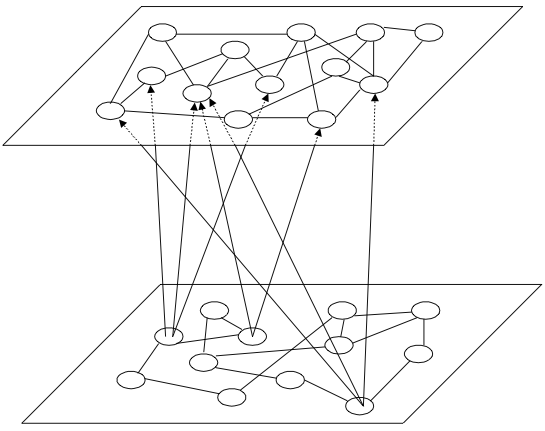
\includegraphics[width=0.5\textwidth]{../graphics/graph-layers}}                
  \subfloat[]{\label{fig:graph-layers-detail}
    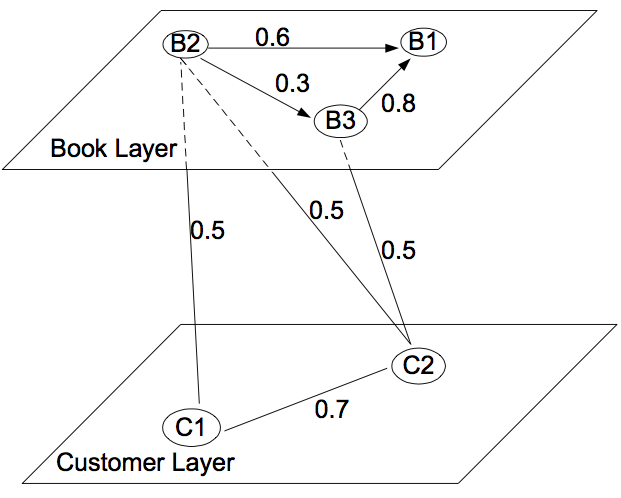
\includegraphics[width=0.5\textwidth]{../graphics/graph-layers-detail}}
  \caption[Network Traversal]{Network Traversal: (a) A graph with two kinds of nodes,
    e.g. items and users. (b) A graph with books and customers, where recommendations
    can be made by traversing the weighted connections. Connections between nodes of the same type
    represent similarity, while connections between books and customers represent purchases.
    Figures from \cite{Huang2002}.}
  \label{fig:book-graphs}
\end{figure}

The complexity of recommender systems based on networks are only limited by the kinds of relations we can produce.
For example, recommending other users in social networks can easily utilize friend or friend-of-a-friend relations
to find others the current user might be interested in connecting to. Indeed, any relevant similarity metric can be used to
connect nodes of the same type, or nodes of different types.

One variation comes from \cite{Walter2008}, who create a network of \emph{transitive trust} to produce recommendations. Here,
the neighborhood of users is determined by traversing through users connected by a level of trust. 
The trust can for example be a function of how many agreeable results the connection to a user has produced.
In other words, users trust each others recommendations based on previous experience.

\cite{Konstas} takes yet another approach that measures the similarity between two nodes through their \emph{random walks with restarts} (RWR) technique.

Starting from a node $x$, the RWR algorithm randomly follows a link to a neighboring node. 
In every step, there is a probability $\alpha$ that the algorithm will restart its random walk from the same node, $x$. 
A user-specific column vector $\mathbf{p}^{(t)}$ stores the long term probability rates of each node, 
where $\mathbf{p}^{(t)}_i$ represents the probability that the random walk at step $t$ is at node $i$. 
$\mathbf{S}$ is the column-normalized adjacency-matrix of the graph, i.e. the transition probability table. 
$\mathbf{q}$ is a column vector of zeroes with a value of $1$ at the starting node (that is, $\mathbf{q}_i$ is $1$ when the RWR algorithm starts at node $x$). 
The stationary probabilities of each node, signifying their long term visiting rate, is then given by 

\begin{equation*}
  \mathbf{p}^{(t+1)} = (1 - \alpha)\mathbf{S}\mathbf{p}^{(t)} + {\alpha}\mathbf{q}
\end{equation*}

when it is run to convergence (within a small delta). Then, the \emph{relatedness} of nodes $x$ and $y$ is given by $\mathbf{p}_y$ where $p$ is the user model for the user represented by node $x$.
\citeauthor{Konstas} found that this approach outperformed the PCC, as long as the social networks were an explicit part of the system in question.
In other words, the connections between users had to be one actively created by the users to be of such quality and precision that
accurate predictions could be made.

After this whirlwind tour of recommender systems, it is time to look at some closely related topics:
information retrieval and personalized search. This will form the basis for the case study
performed in the next chapter.

